\documentclass{article}
\usepackage[margin=1in]{geometry}
\usepackage{fancyhdr}
\usepackage{graphicx}
\usepackage{vhistory}
\usepackage[parfill]{parskip}
\graphicspath{{../Images/}}

% Set fancy looking header/footer and move page number to the right
\pagestyle{fancy}
\fancyhead{}
\fancyfoot{}
\fancyfoot[R]{\thepage}

\title{}
\author{}
\date{}

\begin{document}
    \pagenumbering{gobble}
    \begin{titlepage}
    \begin{center}
        \vspace*{1cm}

        \Huge
        \textbf{User's Guide for Cloud Backup}

        \vspace{.5cm}
        \LARGE
        Captain CyBeard: Neil Before Us

        \vspace{1cm}

        \textbf{Ryan Breitenfeldt \textbar\ Noah Farris\\ Trevor Surface \textbar\ Kyle Thomas}

        \vspace{.2cm}
        \Large
        May 4, 2020

        \vspace{2cm}
        
\includegraphics[scale=1]{logo}

        \vfill

        Washington State University Tri-Cities\\
        CptS 423 Software Design Project 2

    \end{center}
\end{titlepage}



    \listoffigures

    \newpage
    \pagenumbering{arabic}

    \begin{figure}[h]
    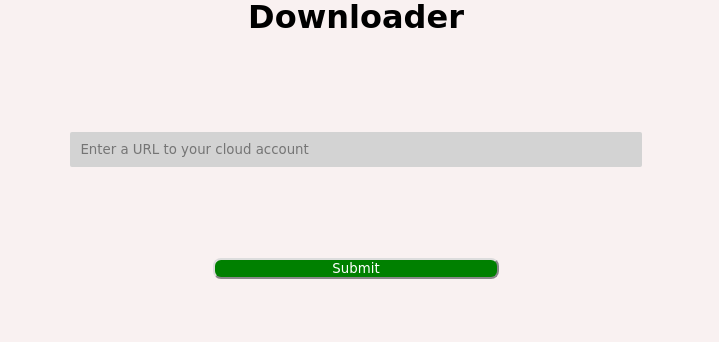
\includegraphics[scale=.7]{s0}
        \caption{First page, ready for a url to a cloud platform.}
    \end{figure}

    \begin{figure}[h]
    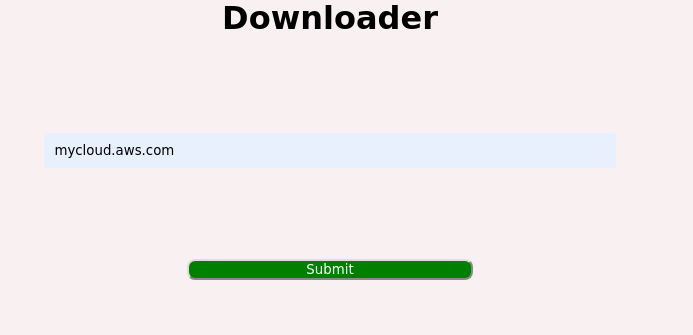
\includegraphics[scale=.7]{s1}
        \caption{URL entered that goes to cloud account.}
    \end{figure}

    \begin{figure}[h]
    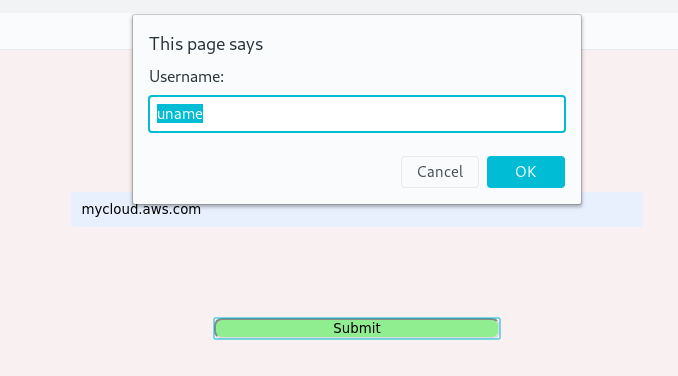
\includegraphics[scale=.7]{s2}
        \caption{Username to cloud platform entered.}
    \end{figure}

    \begin{figure}[h]
    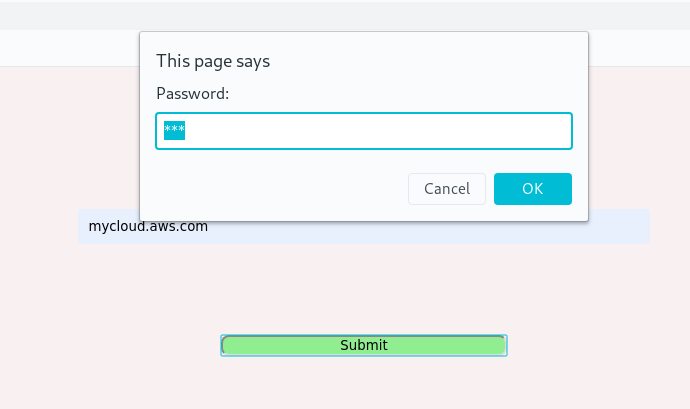
\includegraphics[scale=.7]{s3}
        \caption{Password to cloud platform entered. Note: Javascript doesn't allow for a popup with two text boxes, the actual implementation
            will include both the username and password entry boxes in the same window.}
    \end{figure}

    \begin{figure}[h]
    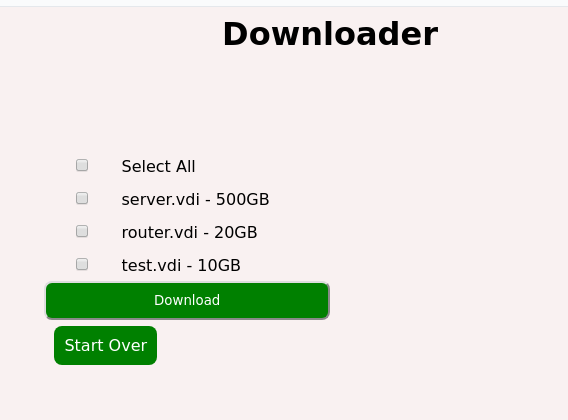
\includegraphics[scale=.7]{s4}
        \caption{Files available for downloading in the root directory of the cloud storage.}
    \end{figure}

    \begin{figure}[h]
    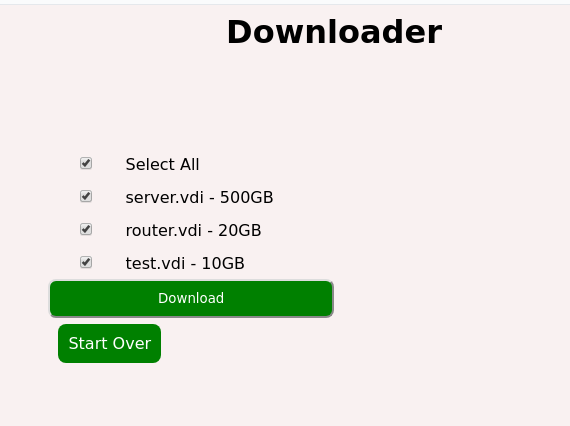
\includegraphics[scale=.7]{s5}
        \caption{All files selected for downloading.}
    \end{figure}

    \begin{figure}[h]
    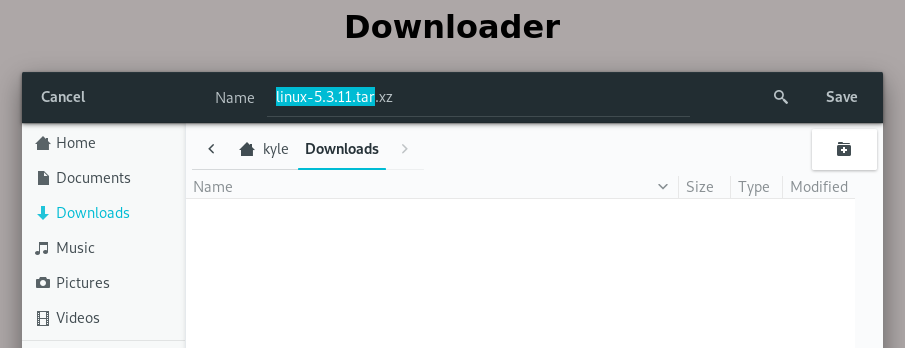
\includegraphics[scale=.5]{s6}
        \caption{Download button pressed, browser prompts where to save files.}
    \end{figure}

\end{document}
